\documentclass[spanish]{beamer}

%Language symbols
\usepackage[spanish]{babel}
\selectlanguage{spanish}
\usepackage[utf8]{inputenc}
\usepackage{verbatim}

\usepackage{graphicx}
\usepackage{subfig}

% Code

\usepackage{listings,textcomp}
\lstset{
  breakatwhitespace,
  language=c++,
  columns=fullflexible,
  keepspaces,
  breaklines,
  tabsize=2, 
  showstringspaces=false,
  extendedchars=true,
  basicstyle=\fontfamily{pcr}\selectfont\scriptsize,
  keywordstyle=\color{orange},
  upquote=true,
  literate={-}{-}1}

%Theme
\usetheme{metropolis}

%Title
\title{Aplicación del algoritmo Divide y Vencerás}
\date{\today}
\author{Yábir G. Benchakhtir}
\institute{Doble Grado en Ingeniería Informática y Matemáticas}
%Document
\begin{document}

\frame{\titlepage}

\begin{frame}\frametitle{Descripción del problema}

  Para poner en práctica este algoritmo se nos presenta inicialmente un
  vector de números comprendido en un intervalo $[-M, M]$ de modo que se
  escojen numeros de manera aleatoria de ese intervalo y se crea un
  vector de un tamaño $N$. Posteriormente se aplica el algoritmo sort
  que incorporla la libería \textit{algorithm} de \textit{C++}.

  Bajo esta hipótesis tenemos que crear un algoritmo de manera que
  encontremos, si existe, un elemento del vector(\textit{v}) tal que
  $v[i] = i$.

  
\end{frame}

\begin{frame}[fragile]\frametitle{Primer algoritmo}
\begin{lstlisting}
int inpos(vector<int> &v){
  int min = 0;
  int max = v.size();
  int mid;

  while (min <= max){
    mid = (max+min)/2;
    
    if (v[mid] == mid)
      return mid;
    else if(v[mid] < mid)
      min = mid + 1;
    else if(v[mid] > mid)
      max = mid-1; 
  }

  return -1;
}
\end{lstlisting}
\end{frame}

\begin{frame}[fragile]\frametitle{Comparación}

\begin{lstlisting}
int inposOdd(vector<int> v){

  int i;

  for(i = 0; i < v.size(); i++)
    if(v[i] == i)
      return i;

  return -1;
}
\end{lstlisting}
\end{frame}

\begin{frame}\frametitle{Contexto}

El programa descrito se ha compilado usando \textit{g++} en su versión
\textit{g++ (Ubuntu 5.4.0-6ubuntu1~16.04.9) 5.4.0 20160609} en una máquina con las siguientes especificaciones:


\begin{itemize}
\item CPU: Intel Pentium G3258 (2) @ 3.200GHz
\item Memoria RAM: 7876MiB
\item Kernel: 4.13.0-36-generic
\item OS: Linux Mint 18.3 Sylvia x86\_64
\end{itemize}

  
\end{frame}

\begin{frame}[fragile]\frametitle{Resultados}
  \begin{figure}[H]
  \centering   
      \subfloat{%
        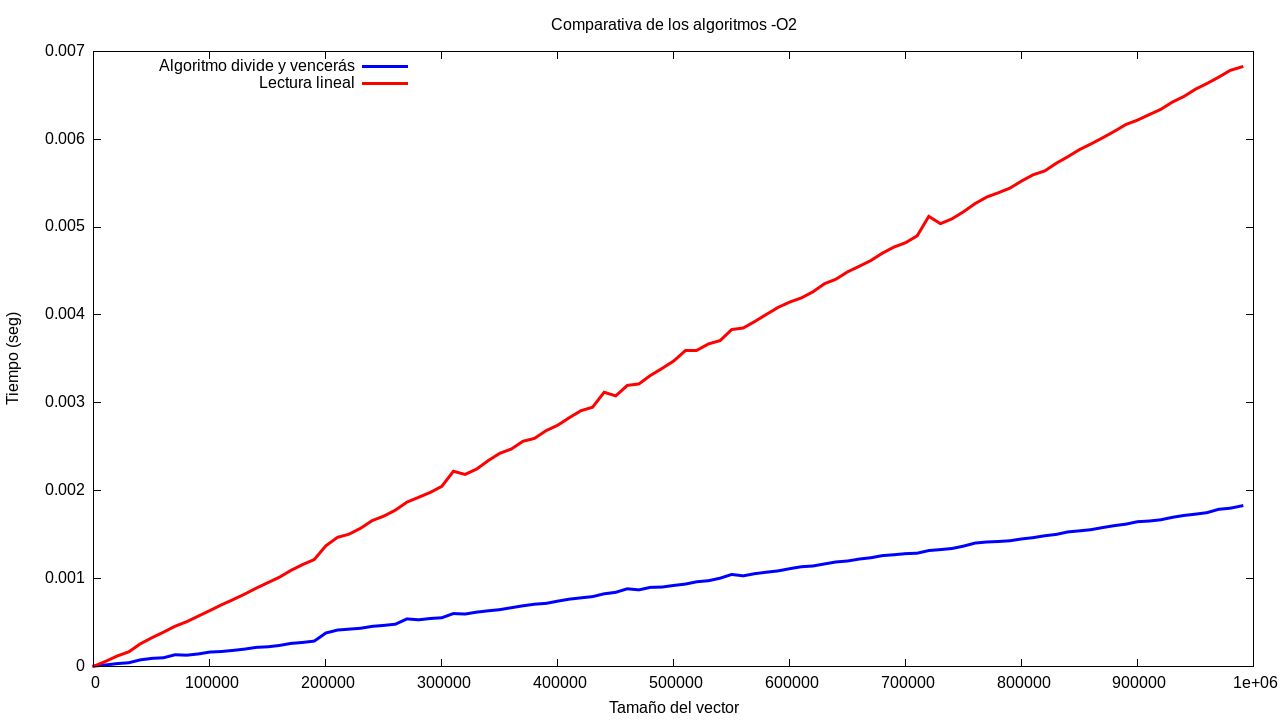
\includegraphics[clip,width=1\columnwidth]{../plots/copia_4.png}%
      }
    \end{figure}
  \end{frame}

  
\begin{frame}[fragile]\frametitle{Eficiencia híbrida $log(n)$}
  \begin{figure}[H]
  \centering   
      \subfloat{%
        \includegraphics[clip,width=1\columnwidth]{../plots/hibrida2.png}%
      }
    \end{figure}
  \end{frame}

\footnotesize %change the font size. You can \scriptsize to get a smaller font.
\begin{frame}[fragile]
  \[f(x) = blog(x+c)+a\]
  
\begin{verbatim}
Final set of parameters            Asymptotic Standard Error
=======================            ==========================

a               = -0.189463        +/- 0.02642      (13.95%)
b               = 0.0121242        +/- 0.001582     (13.05%)
c               = 6.10404e+06      +/- 8.595e+05    (14.08%)
\end{verbatim}
\end{frame}

\begin{frame}[fragile]\frametitle{Eficiencia híbrida $mx+n$}
  \begin{figure}[H]
  \centering   
      \subfloat{%
        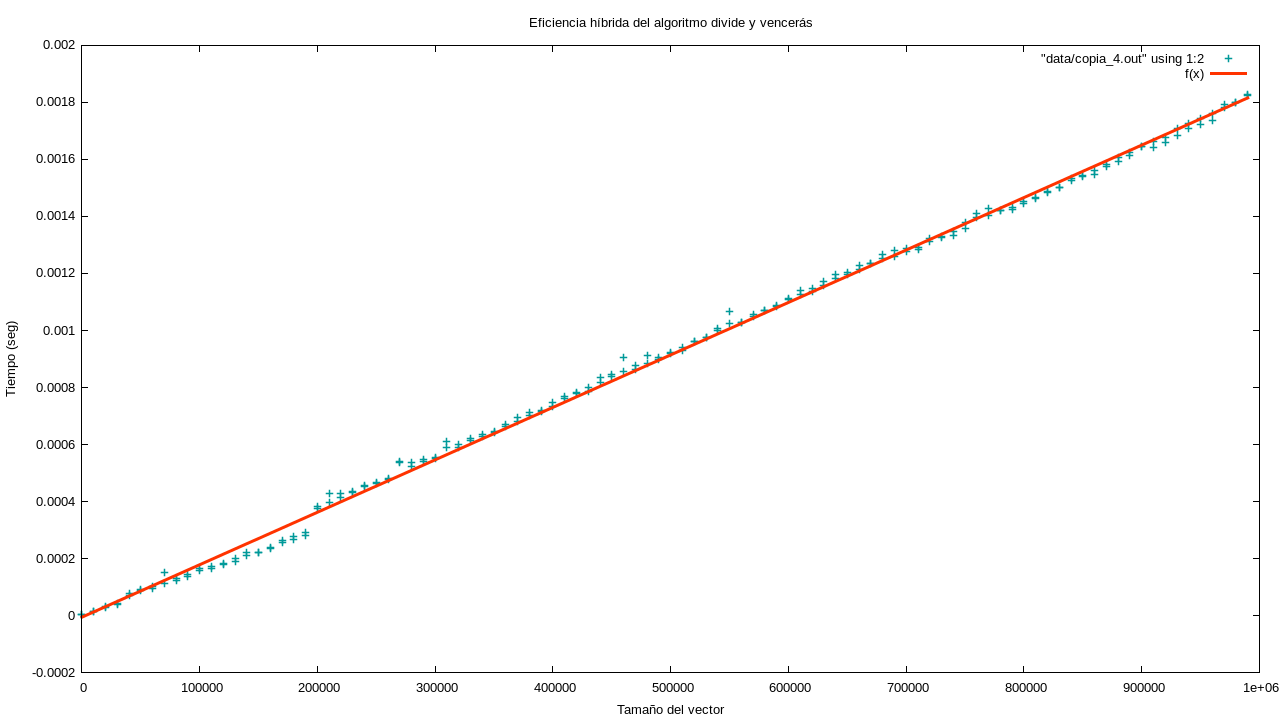
\includegraphics[clip,width=1\columnwidth]{../plots/hibrida_lineal.png}%
      }
    \end{figure}
  \end{frame}

\footnotesize %change the font size. You can \scriptsize to get a smaller font.
\begin{frame}[fragile]
  \[f(x) = bx+a\]
  
\begin{verbatim}
Final set of parameters            Asymptotic Standard Error
=======================            ==========================

a               = -5.18976e-06     +/- 2.963e-06    (57.1%)
b               = 1.83948e-09      +/- 5.171e-12    (0.2811%)
\end{verbatim}
\end{frame}

\begin{frame}[fragile]\frametitle{Mejora de nuestro algoritmo}

  \begin{lstlisting}
int conRepetidos(vector<int> &v, int top, int bot){

  if (bot > top)
    return -1;

  int mid = (top+bot)/2;
  int midv = v[mid];

  if (midv == mid)
    return mid;

  int lefti = min(mid-1, midv);
  int left  = conRepetidos(v, lefti, bot);

  if (left != -1)
    return left;

  int righti = max(mid+1, midv);
  int right = conRepetidos(v, bot, top);

  return right;
      
}
\end{lstlisting}
\end{frame}

\begin{frame}[fragile]\frametitle{Una primera implementación}
  \begin{lstlisting}
  int inpos(int T[], int init, int len){
  int mid = len/2;
  
  if(len != 0){
    if (T[init + mid] == init+mid )
      return init+mid;
    else{
      int below = inpos(T, init, mid);
      int up = inpos(T, init + mid+1, len - mid-1);

      if(below != -1)
	return below;
      if (up != -1)
	return up;	  
    }
  }

  return -1;
}
\end{lstlisting}
\end{frame}

\begin{frame}[fragile]

  \begin{figure}[H]
  \centering   
      \subfloat{%
        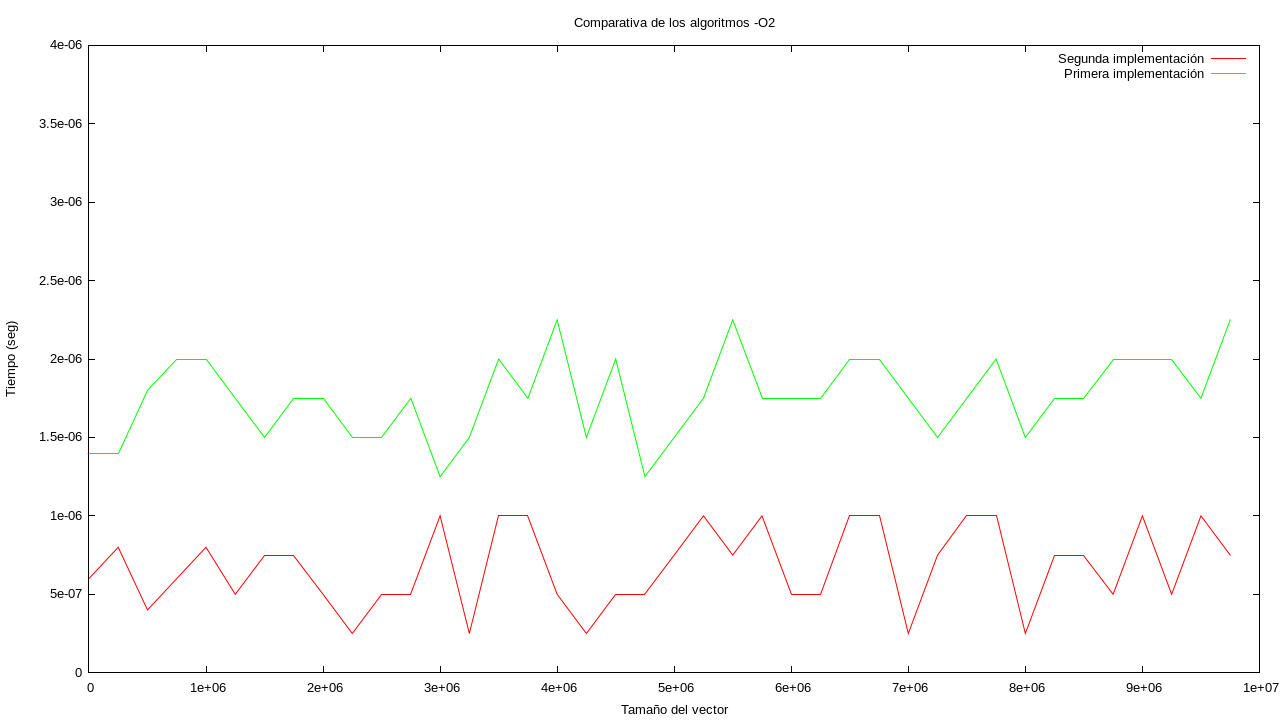
\includegraphics[clip,width=1\columnwidth]{../plots/segundoDyV.png}%
      }

\caption{Comparación de ambos algoritmos DyV}
\end{figure}
  
\end{frame}

\end{document}

